% Created 2020-06-04 Thu 21:25
% Intended LaTeX compiler: pdflatex
\documentclass[presentation]{beamer}
\usepackage[utf8]{inputenc}
\usepackage[T1]{fontenc}
\usepackage{graphicx}
\usepackage{grffile}
\usepackage{longtable}
\usepackage{wrapfig}
\usepackage{rotating}
\usepackage[normalem]{ulem}
\usepackage{amsmath}
\usepackage{textcomp}
\usepackage{amssymb}
\usepackage{capt-of}
\usepackage{hyperref}
\usepackage{minted}
\usepackage[utf8]{inputenc}
\usepackage{color}
\usetheme[height=7mm]{Rochester}
\setbeamertemplate{footline}[frame number]
\usecolortheme[accent=red, light]{solarized}
\setbeamercolor{frametitle}{bg=solarizedRebase02,fg=solarizedAccent}
\setbeamercolor{author in head/foot}{bg=solarizedRebase02,fg=solarizedRebase01}
\setbeamercolor{title in head/foot}{bg=solarizedRebase02,fg=solarizedRebase01}
\setbeamercolor{block title}{bg=solarizedRebase0,fg=solarizedRebase02}
\setbeamercolor{block body}{bg=solarizedRebase02,fg=solarizedRebase0}
\setbeamercolor{item}{bg=solarizedRebase02,fg=solarizedAccent}
\beamertemplatenavigationsymbolsempty
\usemintedstyle{manni}
\AtBeginSection[]{
\begin{frame}
\vfill
\centering
\begin{beamercolorbox}[sep=8pt,center,shadow=true,rounded=true]{title}
\Huge\insertsectionhead\par%
\end{beamercolorbox}
\vfill
\end{frame}
}
\usetheme{default}
\author{Sebastian Stabinger}
\date{SS2020}
\title{Einführung in C++: Strings, Vektoren, \ldots{}}
\hypersetup{
 pdfauthor={Sebastian Stabinger},
 pdftitle={Einführung in C++: Strings, Vektoren, \ldots{}},
 pdfkeywords={},
 pdfsubject={},
 pdfcreator={Emacs 26.3 (Org mode 9.1.9)}, 
 pdflang={Ger}}
\begin{document}

\maketitle

\section{Strings}
\label{sec:org17bb6ed}
\begin{frame}[fragile,label={sec:org45a4c14}]{Strings in C}
 \begin{itemize}
\item Ein Array vom Typ {\color{solarizedYellow}\texttt{char}}
\item Wir müssen uns selbst um die Größe kümmern
\item Ende des Strings ist durch das Zeichen {\color{solarizedYellow}\texttt{\textbackslash{}0} }gekennzeichnet
\end{itemize}
\begin{block}{Beispiel für einen C String im Speicher}
\begin{minted}[fontsize=\scriptsize,numberblanklines=false]{c++}
char str[] = "PROGRAM";
\end{minted}
\begin{center}\begin{center}
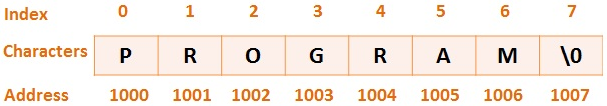
\includegraphics[width=.9\linewidth]{data/cb/fcc991-bddd-49c7-a9fb-fff24aa41a8b/screenshot-20160221-203103.png}
\end{center}\end{center}
\end{block}
\end{frame}
\begin{frame}[fragile,label={sec:org17a9e47}]{Strings in C: Ein Beispiel}
 Wir wollen den Inhalt von zwei Strings {\color{solarizedYellow}\texttt{str1} }und {\color{solarizedYellow}\texttt{str2}}
aneinanderhängen und das Ergebnis in {\color{solarizedYellow}\texttt{str3} }speichern.
\begin{exampleblock}{Beispiel}
\begin{minted}[fontsize=\scriptsize,numberblanklines=false]{c}
#include <stdio.h>
#include <string.h>

// Wir müssen uns selbst darum kümmern, dass str3 groß genug ist
char str1[100], str2[100], str3[200];
strcpy(str1, "Hello ");
// str1 = "Hello " funktioniert nicht!
strcpy(str2, "World");
// Hänge str1 und str2 zusammen und speichere in str3
strcpy(str3, str1);
strcat(str3, str2);
// Gib str3 auf Bildschirm aus
printf("%s", str3);  // Wir müssen den Typ von str3 angeben (%s)
\end{minted}
\end{exampleblock}
Man sieht: Die Verwendung ist \alert{umständlich und unnatürlich}
\end{frame}
\begin{frame}[fragile,label={sec:org07fdfe0}]{Strings in C++}
 \begin{itemize}
\item Ein eigener Datentyp names {\color{solarizedYellow}\texttt{std::string}}
\item Die Größe wird dynamisch angepasst
\item Verhält sich wie man es erwarten würde!
\end{itemize}
\begin{exampleblock}{Beispiel}
\begin{minted}[fontsize=\scriptsize,numberblanklines=false]{c++}
#include <iostream>
#include <string>
using namespace std;

string str1, str2, str3; // Platz für beliebig viele Zeichen
str1 = "Hello ";         // Wir können einfach zuweisen
str2 = "World";
// Hänge str1 und str2 zusammen und speichere in str3
str3 = str1 + str2;
// Gib str3 auf Bildschirm aus
cout << str3 << endl; // Der Compiler kennt den Typ!
\end{minted}
\end{exampleblock}
\begin{itemize}
\item Falls wir z.B. {\color{solarizedYellow}\texttt{str3} }als C-String benötigen:  {\color{solarizedYellow}\texttt{str3.c\_str()}}
\end{itemize}
\end{frame}
\begin{frame}[fragile,label={sec:org5e95dc0}]{Vergleichen von Strings}
 Um zu testen, ob zwei Strings gleich sind muss in C eine spezielle
Funktion ({\color{solarizedYellow}\texttt{strcmp}}) verwendet werden. In C++ erfolgt der Vergleich
ganz natürlich mit dem Vergleichsoperator {\color{solarizedYellow}\texttt{==}}, wie bei allen anderen
Datentypen auch.
\begin{exampleblock}{C}
\begin{minted}[fontsize=\scriptsize,numberblanklines=false]{c}
if (strcmp(str1, str2) == 0) {
  printf("String 1 und 2 sind gleich");
}
\end{minted}
\end{exampleblock}
\begin{exampleblock}{C++}
\begin{minted}[fontsize=\scriptsize,numberblanklines=false]{c++}
if (str1 == str2) {
  std::cout << "String 1 und 2 sind gleich";
}
\end{minted}
\end{exampleblock}
\end{frame}
\begin{frame}[fragile,label={sec:org529e2b2}]{Konvertierungen}
 \begin{block}{\ldots{} in einen String}
Zahlen können mittels der Funktion {\color{solarizedYellow}\texttt{to\_string} }in einen {\color{solarizedYellow}\texttt{string}}
konvertiert werden.
\begin{minted}[fontsize=\scriptsize,numberblanklines=false]{c++}
string s = to_string(42);  // s enthält den String "42"
\end{minted}
\end{block}
\begin{block}{\ldots{} von einem String}
Ein String welcher eine Zahl enthält kann mit folgenden Funktionen in
eine Zahl konvertiert werden:
\begin{itemize}
\item {\color{solarizedYellow}\texttt{stoi}}, {\color{solarizedYellow}\texttt{stol}}, {\color{solarizedYellow}\texttt{stoll} }für Integer, Long und Long Long
\item {\color{solarizedYellow}\texttt{stof}}, {\color{solarizedYellow}\texttt{stod}}, {\color{solarizedYellow}\texttt{stold} }für Float, Double und Long Double
\end{itemize}
\begin{minted}[fontsize=\scriptsize,numberblanklines=false]{c++}
int i = stoi("42"); // i enthält die Zahl 42
\end{minted}
\end{block}
Für komplexere Umwandlungen verwendet man einen {\color{solarizedYellow}\texttt{stringstream}}.
\end{frame}
\begin{frame}[fragile,label={sec:org9eddb90}]{Daten formatieren mit {\color{solarizedYellow}\texttt{stringstream} }[optional]}
 \begin{itemize}
\item Man erzeugt einen \alert{String Stream} mittels {\color{solarizedYellow}\texttt{stringstream} }(benötigt
{\color{solarizedYellow}\texttt{sstream} }als Include)
\item Schreiben wie in {\color{solarizedYellow}\texttt{cout}}
\item Um daraus einen String zu erzeugen: {\color{solarizedYellow}\texttt{.str()}}
\end{itemize}
\begin{exampleblock}{Beispiel}
\begin{minted}[fontsize=\scriptsize,numberblanklines=false]{c++}
#include <iostream>
#include <sstream>
using namespace std;

int main() {
  stringstream str_stream;
  str_stream << "Die Antwort ist " << 42 << " !";
  string str = str_stream.str();

  cout << str << endl;
} // Ausgabe: Die Antwort ist 42 !
\end{minted}
\end{exampleblock}
\end{frame}
\begin{frame}[fragile,label={sec:org525737b}]{Daten extrahieren mit {\color{solarizedYellow}\texttt{stringstream} }[optional]}
 \begin{itemize}
\item {\color{solarizedYellow}\texttt{stringstream ss(string)} }erzeugt einen Stringstream namens {\color{solarizedYellow}\texttt{ss} }aus
einem bereits existierenden String.
\item Aus einem {\color{solarizedYellow}\texttt{stringstream} }können wie mittels {\color{solarizedYellow}\texttt{cin} }Daten ausgelesen
werden
\end{itemize}
\begin{exampleblock}{Beispiel}
\begin{minted}[fontsize=\scriptsize,numberblanklines=false]{c++}
#include <iostream>
#include <sstream>
#include <string>
using namespace std;

int main() {
  string s = "23 42 47";
  stringstream str_stream(s); // oder direkt str_stream("23 42 47")
  int a, b, c;
  str_stream >> a >> b >> c; // Einlesen der Daten

  cout << "a=" << a << " b=" << b << " c=" << c << endl;
} // Ausgabe: a=23 b=42 c=47
\end{minted}
\end{exampleblock}
\end{frame}

\section{\texttt{vector} als Array-Alternative}
\label{sec:org99c1e23}
\begin{frame}[fragile,label={sec:org71ba744}]{Fundamentale Arrays --- Einige Probleme}
 \begin{block}{Größe ist nicht Teil des Datentyps}
\begin{minted}[fontsize=\scriptsize,numberblanklines=false]{c++}
int sum(int *a, int length) {
  // Länge muss explizit mitgegeben werden
  int sum = 0;
  for (int i = 0; i < length; i++) {
    sum += a[i];
  }
  return sum;
}
\end{minted}
\end{block}
\begin{block}{Keine Überprüfung von Indexfehlern}
\begin{minted}[fontsize=\scriptsize,numberblanklines=false]{c++}
int a[10];
a[20] = 47; // Ouch! Kein Fehler!!
\end{minted}
\end{block}
\begin{itemize}
\item Die Größe muss vorab bekannt sein wenn man nicht dynamische
Speicherverwaltung verwenden will!
\end{itemize}
\end{frame}
\begin{frame}[fragile,label={sec:org3585a98}]{{\color{solarizedYellow}\texttt{vector} }--- Die C++ Alternative}
 Verwendbar mittels {\color{solarizedYellow}\texttt{\#include <vector>}}

Vorteile:
\begin{itemize}
\item Automatisches Speichermanagement
\item Dynamische Größe
\item Überprüft auf Indexfehler (wenn man das will)
\item Bietet viele komfortable Funktionen
\end{itemize}
\begin{exampleblock}{Arraybeispiel mit {\color{solarizedYellow}\texttt{vector} }implementiert}
\begin{minted}[fontsize=\scriptsize,numberblanklines=false]{c++}
vector<int> a(100); // Vektor mit Platz für 100 Integer Werte
// Vektor mit den Zahlen 1 bis 5
vector<int> b = {1, 2, 3, 4, 5};
// Ausgabe des ersten Elements von a und fünften von b
cout << "a[0]=" << a[0] << " b[4]=" << b[4] << endl;
// Ausgabe: a[0]=0 b[4]=5
\end{minted}
\end{exampleblock}
\end{frame}
\begin{frame}[fragile,label={sec:org130eca2}]{{\color{solarizedYellow}\texttt{vector} }mit bekannter Größe}
 Ein Vektor mit bekannter Größe kann folgendermaßen deklariert werden: {\color{solarizedYellow}\texttt{vector<typ> name(größe);}}
\begin{exampleblock}{Beispiel}
\begin{minted}[fontsize=\scriptsize,numberblanklines=false]{c++}
vector<int> a(100); vector<double> bla(400);
\end{minted}
\end{exampleblock}
Im Gegensatz zu einem Fundamentalen Array kann die Größe aber auch
erst \alert{zur Laufzeit} festgelegt werden. D.h. \alert{als Größe kann auch eine
Variable} angegeben werden (in C seit C99 auch möglich) und die
\alert{Größe} kann problemlos \alert{zur Laufzeit verändert werden}.
\begin{exampleblock}{Beispiel}
Angenommen {\color{solarizedYellow}\texttt{get\_num} }fragt den Benutzer nach einer Zahl und gibt
diese zurück
\begin{minted}[fontsize=\scriptsize,numberblanklines=false]{c++}
int size = get_num();
vector<int> vec(size);
// vec hat die Größe welche der Benutzer eingegeben hat
\end{minted}
\end{exampleblock}
\end{frame}
\begin{frame}[fragile,label={sec:orgeec5c98}]{Der leere Vektor}
 Für die Verwendung von {\color{solarizedYellow}\texttt{vector} }muss die benötigte \alert{Größe nicht von
Anfang an bekannt sein}. Wir lassen die Größe einfach weg und erzeugen
damit einen leeren Vektor: {\color{solarizedYellow}\texttt{vector<typ> name;}}
\begin{exampleblock}{Beispiel}
\begin{minted}[fontsize=\scriptsize,numberblanklines=false]{c++}
vector<int> a; vector<double> bla;
\end{minted}
\end{exampleblock}
\begin{alertblock}{Vorsicht!}
Sie dürfen nicht auf Elemente eines Vektors zugreifen wenn diese nicht
existieren!
\begin{minted}[fontsize=\scriptsize,numberblanklines=false]{c++}
vector<int> a; // Vektor hat Größe 0
a[0] = 10; // Im besten Fall ein Speicherfehler ...
cout << a[0] << endl; // ... im ungünstigsten Fall unvorhersehbar
\end{minted}
\end{alertblock}
\end{frame}
\begin{frame}[fragile,label={sec:orgb3a0a93}]{Wofür ein leerer Vektor?}
 Wenn man nicht auf Elemente eines leeren Vektors zugreifen kann, wofür
ist er dann nützlich?
\begin{exampleblock}{Späteres Festlegen der Größe mit {\color{solarizedYellow}\texttt{resize}}}
\begin{minted}[fontsize=\scriptsize,numberblanklines=false]{c++}
vector<int> a;
a.resize(100); // Vektor a hat jetzt Platz für 100 Integer
a.resize(200); // Vektor a hat jetzt Platz für 200 Integer
\end{minted}
\end{exampleblock}
\begin{exampleblock}{Anhängen von Elementen mit {\color{solarizedYellow}\texttt{push\_back}}}
\begin{minted}[fontsize=\scriptsize,numberblanklines=false]{c++}
vector<int> a;
a.push_back(12);
a.push_back(23);
a.push_back(42);
// a enthält nun {12, 23, 42}
\end{minted}
\end{exampleblock}
\end{frame}
\begin{frame}[fragile,label={sec:org40fd98f}]{Zugriff auf Elemente}
 \begin{minted}[fontsize=\scriptsize,numberblanklines=false]{c++}
vector<int> vec;
vec.push_back(23); vec.push_back(42); vec.push_back(7);
\end{minted}
\begin{block}{Ohne Bounds Checking (schneller)}
Funktioniert wie bei Arrays mittels {\color{solarizedYellow}\texttt{[index]}}
\begin{minted}[fontsize=\scriptsize,numberblanklines=false]{c++}
vec[0]; // == 23
vec[2]; // == 7
vec[5]; // == ?? keinerlei Garantien
\end{minted}
\tiny VisualStudio macht bei Debug Builds auch hier ein Bounds
Checking! Kann bei den meinsten Compilern eingestellt werden (z.B. für
gcc mit dem Compilerflag {\color{solarizedYellow}\texttt{-D\_GLIBCXX\_DEBUG}})
\end{block}
\begin{block}{Mit Bounds Checking (sicherer)}
Mit Hilfe der Funktion {\color{solarizedYellow}\texttt{.at(index)}}
\begin{minted}[fontsize=\scriptsize,numberblanklines=false]{c++}
vec.at(0); // == 23
vec.at(2); // == 7
vec.at(5); // Wirft zur Laufzeit zuverlässig eine Exception
\end{minted}
\end{block}
Beide Versionen können auch für die Zuweisung von Werten verwendet
werden: {\color{solarizedYellow}\texttt{vec[1] = 10;} }bzw. {\color{solarizedYellow}\texttt{vec.at(1) = 10;}}
\end{frame}
\begin{frame}[fragile,label={sec:org3f91e66}]{Löschen von Elementen}
 \begin{itemize}
\item Es ist möglich \alert{einzelne Elemente} aus einem Vektor mit folgender
Funktion zu \alert{löschen}:
\end{itemize}
{\color{solarizedYellow}\texttt{vektorname.erase(vektorname.begin() + position)}}
\begin{itemize}
\item Falls ein anderes Element als das letzte im Vektor gelöscht wird ist
die Operation \alert{relativ langsam} ({\color{solarizedYellow}\texttt{list} }ist für solche Fälle eine
bessere Alternative zu {\color{solarizedYellow}\texttt{vector}})
\item In den meisten Fällen aber trotzdem \alert{schnell genug}!

\item 
\end{itemize}
\end{frame}

\begin{frame}[fragile,label={sec:org017091e}]{Löschen von Elementen --- Beispiel}
 \begin{block}{Beispiel}
\begin{minted}[fontsize=\scriptsize,numberblanklines=false]{c++}
#include <iostream>
#include <vector>
using namespace std;

int main() {
  vector<int> vec = {2, 6, 1, 28, 42, 23, 47, 7};

  vec.erase(vec.begin() + 3);

  for (int &i : vec)
    cout << i << " ";
}
\end{minted}
\end{block}

\begin{block}{Ausgabe}
\begin{verbatim}
2 6 1 42 23 47 7
\end{verbatim}
\end{block}
\end{frame}

\begin{frame}[fragile,label={sec:org51bc006}]{Weitere Nützliche Funktionen}
 \begin{itemize}
\item {\color{solarizedYellow}\texttt{.size()} }Gibt die Anzahl an Elementen zurück
\item {\color{solarizedYellow}\texttt{.empty()} }Gibt {\color{solarizedYellow}\texttt{true} }zurück falls der Vektor keine Elemente enthält
\item {\color{solarizedYellow}\texttt{.data()} }Gibt ein C-Array auf die Daten des Vektors zurück. Wichtig
falls man mit C-Code interagieren muss.
\item {\color{solarizedYellow}\texttt{.pop\_back()} }Löscht das letzte Element vom Vektor. Gegenstück zu
{\color{solarizedYellow}\texttt{.push\_back(element)}}.
\item {\color{solarizedYellow}\texttt{.back()} }Gibt letztes Element des Vektors zurück ohne es zu löschen
\item {\color{solarizedYellow}\texttt{==} }Zwei Vektoren können mittels {\color{solarizedYellow}\texttt{==} }verglichen werden. Die
Vektoren gelten als gleich falls sie die gleiche Größe haben und die
selben Elemente enthalten. {\color{solarizedYellow}\texttt{if(vec1 == vec2);}}
\end{itemize}
\end{frame}
\begin{frame}[fragile,label={sec:org0284bd0}]{Vector --- Beispiel}
 \begin{minted}[fontsize=\scriptsize,numberblanklines=false]{c++}
#include <iostream>
#include <vector>
using namespace std;

int main() {
  vector<int> vec;
  cout << "Größe von vec: " << vec.size() << endl;
  vec.push_back(23);
  vec.push_back(13);
  vec.push_back(42);
  vec.push_back(7);
  cout << "Größe von vec: " << vec.size() << endl;
  // For-each 
  for (auto e : vec)
    cout << e << " ";
}
\end{minted}
\begin{block}{Ausgabe}
\begin{minted}[fontsize=\scriptsize,numberblanklines=false]{text}
Größe von vec: 0
Größe von vec: 4
23 13 42 7 
\end{minted}
\end{block}
\end{frame}
\section{for-each}
\label{sec:org7d98078}
\begin{frame}[fragile,label={sec:orgfcb0c92}]{{\color{solarizedYellow}\texttt{for} }- each (neu in C++11)}
 Iteriert automatisch über alle Elemente eines "Containers" z.B. Array,
Vector, etc.
\begin{block}{Beispiel}
\begin{minted}[fontsize=\scriptsize,numberblanklines=false]{c++}
std::vector<int> vec = {23, 12, 42, 13, -40}; // Ein Array

for (int i : vec) {
  std::cout << i << " ";
}
\end{minted}
\end{block}
\begin{block}{Ausgabe}
\begin{verbatim}
23 12 42 13 -40
\end{verbatim}
\end{block}
\end{frame}
\begin{frame}[fragile,label={sec:org0bcd8ed}]{{\color{solarizedYellow}\texttt{for} }- each --- Zuweisung}
 Um in einer for-each Schleife Werte in ein Array zu schreiben, muss
der Laufvariable ein {\color{solarizedYellow}\texttt{\&} }vorangestellt werden. Dies kennzeichnet die
Variable als eine sogenannte \alert{Referenz} (eine Alternative zu Zeigern
in C++)
\begin{block}{Beispiel 1}
\begin{minted}[fontsize=\scriptsize,numberblanklines=false]{c++}
std::vector<int> vec(100); // Ein Array der Größe 100

// Wir füllen das ganze Array mit dem Wert 23
for (int &i : vec) {
  i = 23;
}
\end{minted}
\end{block}
\end{frame}
\begin{frame}[fragile,label={sec:orgc3d4eb9}]{{\color{solarizedYellow}\texttt{for} }- each --- Zuweisung}
 \begin{block}{Beispiel 2}
\begin{minted}[fontsize=\scriptsize,numberblanklines=false]{c++}
std::vector<int> vec = {1, 2, 3, 4, 5, 6, 7, 8, 9, 10};

// Quadriert alle Einträge in arr
for (int &i : vec) {
  i = i * i;
}

for (int i : vec) {
  std::cout << i << " ";
}
\end{minted}

\begin{verbatim}
1 4 9 16 25 36 49 64 81 100
\end{verbatim}
\end{block}
\end{frame}
\section{Funktionsüberladung}
\label{sec:org237f4ec}
\begin{frame}[fragile,label={sec:org8f91a3b}]{Funktionsüberladung}
 \begin{itemize}
\item Es können mehrere Funktionen mit \alert{gleichem Namen} deklariert werden
so lange die \alert{Datentypen der Argumente eindeutig} sind
\item Der \alert{Compiler wählt die korrekte Funktion} anhand der Datentypen der
an die Funktion übergebenen Argumente aus
\end{itemize}
\begin{block}{OK}
\begin{minted}[fontsize=\scriptsize,numberblanklines=false]{c++}
int f(int a);
double f(double a);
int f(short a);
int f(int a, int b); // Parameteranzahl ist auch wichtig
\end{minted}
\end{block}
\begin{block}{Fehlerhaft}
\begin{minted}[fontsize=\scriptsize,numberblanklines=false]{c++}
int f(int a);
int f(int b); // Error: nur der Typ zählt
double f(int a); // Error: Der Rückgabetyp wird ignoriert
\end{minted}
\end{block}
\end{frame}
\begin{frame}[fragile,label={sec:orgcfd3858}]{Funktionsüberladung --- Beispiel}
 \begin{minted}[fontsize=\scriptsize,numberblanklines=false]{c++}
#include <iostream>

// int wird quadriert
int f(int a) { return a * a; }
// Bei double wird 10 hinzugezählt
double f(double a) { return a + 10; }
// short wird verdoppelt
short f(short a) { return a * 2; }

int main() {
  int a = 5;
  double b = 10;
  short c = 4;

  std::cout << "int: " << f(a) << " ";
  std::cout << "double: " << f(b) << " ";
  std::cout << "short: " << f(c) << " ";
}
\end{minted}
\begin{block}{Ausgabe}
\begin{minted}[fontsize=\scriptsize,numberblanklines=false]{text}
int: 25 double: 20 short: 8
\end{minted}
\end{block}
\end{frame}
\section{\texttt{auto}}
\label{sec:org0a020ee}
\begin{frame}[fragile,label={sec:orgc67a82e}]{{\color{solarizedYellow}\texttt{auto} }(neu in C++11)}
 \begin{itemize}
\item Seit C++11 unterstützt C++ eine einfache Form der sogenannten
\alert{Typinferenz} \footnote{\href{https://de.wikipedia.org/wiki/Typinferenz}{https://de.wikipedia.org/wiki/Typinferenz}}
\item Bedeutet: Falls der Compiler den Typ einer Variable selbst
herausfinden kann, muss man ihn nicht angeben.
\item Um Typinferenz zu verwenden schreibt man {\color{solarizedYellow}\texttt{auto} }statt des
eigentlichen Datentyps.
\end{itemize}
\begin{block}{Beispiel}
\begin{minted}[fontsize=\scriptsize,numberblanklines=false]{c++}
auto i = 10;    // i ist vom Typ int
auto tmp = f(); // tmp hat den Typ welcher von f
                // zurückgegeben wird
\end{minted}
\end{block}
\end{frame}
\end{document}